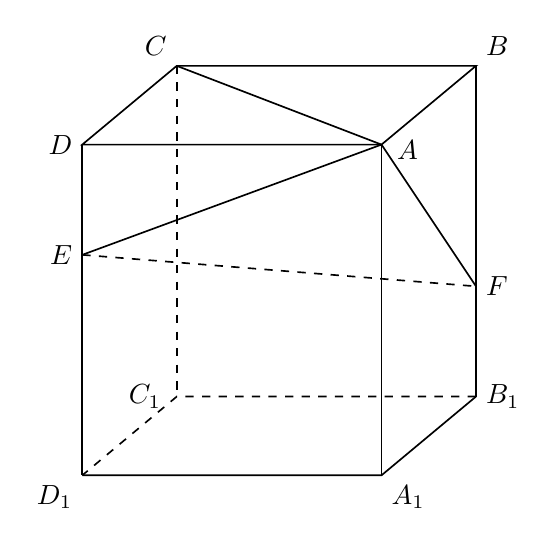
\begin{tikzpicture}[x=1cm,y=1cm,font=\normalsize,line width=.6pt]
\coordinate (D) at (0,4.2);
\coordinate (C) at (1.2,5.2);
\coordinate (B) at (5.0,5.2);
\coordinate (A) at (3.8,4.2);
\coordinate (D1) at (0,0);
\coordinate (C1) at (1.2,1.0);
\coordinate (B1) at (5.0,1.0);
\coordinate (A1) at (3.8,0);
\coordinate (E) at (0,2.8);
\coordinate (F) at (5.0,2.4);
% top face
\draw[solid] (D) -- (C) -- (B) -- (A) -- cycle;
\draw[solid] (C) -- (A);
% verticals
\draw[solid] (D) -- (E);
\draw[solid] (E) -- (D1);
\draw[solid] (A) -- (A1);
\draw[solid] (B) -- (F);
\draw[solid] (F) -- (B1);
\draw[dashed] (C) -- (C1);
% bottom face
\draw[solid] (D1) -- (A1) -- (B1);
\draw[dashed] (B1) -- (C1) -- (D1);
% section triangle AEF
\draw[solid] (A) -- (E);
\draw[solid] (A) -- (F);
\draw[dashed] (E) -- (F);
\node[above left] at (C) {$C$};
\node[above right] at (B) {$B$};
\node[left] at (D) {$D$};
\node[right,xshift=2.00bp,yshift=-2.00bp] at (A) {$A$};
\node[left] at (E) {$E$};
\node[right] at (F) {$F$};
\node[left,xshift=-2.00bp,yshift=0.00bp] at (C1) {$C_{1}$};
\node[right] at (B1) {$B_{1}$};
\node[below left] at (D1) {$D_{1}$};
\node[below right] at (A1) {$A_{1}$};
\end{tikzpicture}
